\documentclass{beamer}

\usepackage{beamerthemesplit}
\usepackage[utf8]{inputenc}
\usecolortheme{rose}
\usepackage{slovak}
\usepackage{subfigure}

\def\languagename{english}
\def\dd{\;{\rm d}\,}
\def\imag{\hat{\imath}}
\def\sipka{\rightarrow}
\def\C{\mathbb{C}}

\def\mytitle{Fourierova transformácia a jej použitie}
\def\myauthor{Peter Perešíni}
\date{\today}
\setbeamercovered{transparent}

\title\mytitle
\author\myauthor

%%% {{{ Section autonumbering
\AtBeginSection[]
{
  \frame<handout:0>
  {
    \frametitle{Prehľad}
%    \tableofcontents[currentsection,hideallsubsections]
    \tableofcontents[sectionstyle=show/shaded,subsectionstyle=show/show/hide]
  }
}
%
%\AtBeginSubsection[]
%{
%  \frame<handout:0>
%  {
%    \frametitle{Prehľad}
%    \tableofcontents[sectionstyle=show/hide,subsectionstyle=show/shaded/hide]
%  }
%}
%%% }}}

\begin{document}

%%% {{{ Title page
\begin{frame}{Obhajoba bakalárskej práce}
    \titlepage
\end{frame}
%%% }}}

%\begin{frame}{Obsah}
%    \tableofcontents
%\end{frame}

%%% {{{ Motivacia
\section{Motivácia}
\begin{frame}{Motivácia}
    \begin{itemize}
        \item dôležitosť v každodennom živote
        \item nekonzistentné zdroje
            \begin{itemize}
                \item rôzne značenia, konvencie, predpoklady
                \item špecifické na konkrétne použitie
                \item neobsahujú súvislosti
            \end{itemize}
        \item Osvojenie si nových poznatkov
    \end{itemize}
\end{frame}
%%% }}}

%%% {{{ Definicie
\section{Fourierova transformácia}
\begin{frame}{Fourierova transformácia}
    \begin{itemize}
        \item 1807 Fourier - "Každá periodická funkcia sa dá vyjadriť
        ako lineárna kombinácia funkcií $\sin kx$ a $\cos kx$,
        $k \in \mathbb{N}_0$"
        \item Prevod medzi dvoma reprezentáciami
            \begin{itemize}
                \item priestorová/časová (štandardná)
                \item frekvenčná (kombinácia harmonických funkcií)
            \end{itemize}
        \item Rôzne formy (Fourierov rad, spojitá FT, diskrétna FT)
    \end{itemize}
\end{frame}

\begin{frame}{Definícia}
    \begin{definition}[Diskrétna Fourierova transformácia]
    $\mathcal{F}:\C^N\sipka\C^N$
        \begin{equation*}
            X_k = \sum_{n=0}^{N-1} x_n e^{\frac{-2\pi\imag}{N} k n}
        \end{equation*}
    \end{definition}
    \begin{definition}[Inverzná transformácia]
        \begin{equation*}
            x_k = \frac{1}{N} \sum_{n=0}^{N-1} X_n e^{\frac{2\pi\imag}{N} kn}
        \end{equation*}
    \end{definition}
\end{frame}
%%% }}}

\section{Použitie}
%%% {{{ Digitalne filtre
\subsection{Digitálne filtre}
\begin{frame}{Digitálne filtre}
    \begin{itemize}
        \item Filtre - základ spracovania signálu
        \item Realizácia filtrov
            \begin{itemize}
                \item Ideálne low/high-pass filtre
                    \begin{itemize}
                    \item v praxi nepoužiteľné
                    \item "zvoniaci" efekt súvisí s Gibbsovým fenoménom
                    \end{itemize}
                \item Hladké filtre - Gaussov, Butterworthov
                \item Ďalšie filtre - korelácia, dekonvolúcia
            \end{itemize}
    \end{itemize}
\end{frame}
%%% }}}

%%% {{{ Gibbsov fenomen
%\begin{frame}{Gibbsov fenomén}
%    \begin{figure}
%        \begin{centering}
%            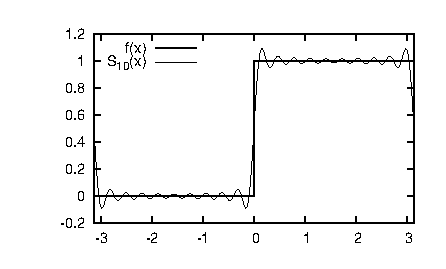
\includegraphics[width=5cm]{obrazky/gibbs_saw10}
%            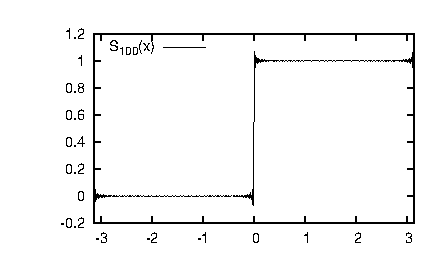
\includegraphics[width=5cm]{obrazky/gibbs_saw100}
%        \end{centering}
%        \caption{Gibbsov fenomén}
%    \end{figure}
%\end{frame}

\begin{frame}{Gibbsov fenomén a zvonenie u ideálnych filtrov}
    \tiny
    \begin{figure}
        \subfigure{}{
            
\includegraphics[width=2cm]{obrazky/source_highpass}
        }
        \\
        \subfigure{}{
            
\includegraphics[width=2cm]{obrazky/ideal_highpass_20}
        }
        \subfigure{Frekvencia}{
            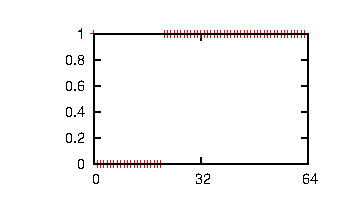
\includegraphics[width=3cm]{obrazky/ideal_highpass_frequency_20}
        }
        \subfigure{Odozva}{
            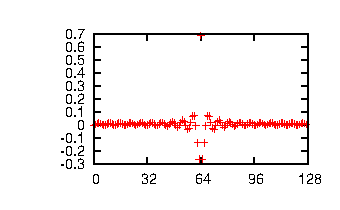
\includegraphics[width=3cm]{obrazky/ideal_highpass_response_20}
        }
        \\
        \subfigure{}{
            
\includegraphics[width=2cm]{obrazky/gauss_highpass_20}
        }
        \subfigure{Frekvencia}{
            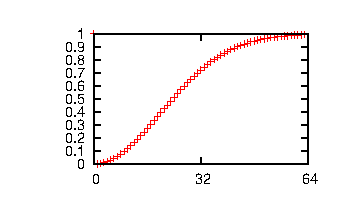
\includegraphics[width=3cm]{obrazky/gauss_highpass_frequency_20}
        }
        \subfigure{Odozva}{
            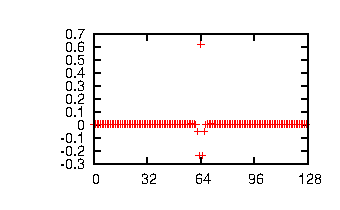
\includegraphics[width=3cm]{obrazky/gauss_highpass_response_20}
        }
    \end{figure}
\end{frame}
%%% }}}

%%% {{{ Faza a magnituda
\subsection{FT - fáza a magnitúda}
\begin{frame}{Súvis medzi fázou a magnitúdou}
    \begin{figure}
        \begin{centering}
        \tiny
        \subfigure{$\phi_1$, mag 1}{
            
\includegraphics[width=2cm]{obrazky/p1m1}
        }
        \subfigure{$\phi_1$, mag 2}{
            
\includegraphics[width=2cm]{obrazky/p1m2}
        }
        \subfigure{$\phi_1$, mag c}{
            
\includegraphics[width=2cm]{obrazky/p1mc}
        }
        \\
        \subfigure{$\phi_2$, mag 1}{
            
\includegraphics[width=2cm]{obrazky/p2m1}
        }
        \subfigure{$\phi_2$, mag 2}{
            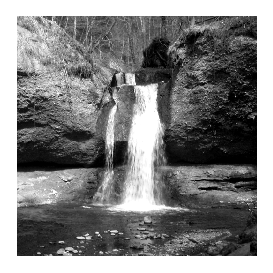
\includegraphics[width=2cm]{obrazky/p2m2}
        }
        \subfigure{$\phi_2$, mag c}{
            
\includegraphics[width=2cm]{obrazky/p2mc}
        }
        \\
        \subfigure{$\phi=0$, mag 1}{
            
\includegraphics[width=2cm]{obrazky/pcm1}
        }
        \subfigure{$\phi=0$, mag 2}{
            
\includegraphics[width=2cm]{obrazky/pcm2}
        }
        \end{centering}
    \end{figure}
\end{frame}
%%% }}}


%%% {{{ Kompresia obrazu a videa
\subsection{Kompresia obrazu}
\begin{frame}{Kompresia obrazu}
    \begin{itemize}
        \item Formát JPEG
        \item Obraz $\sipka$ transformácia $\sipka$ kvantizácia
          $\sipka$ kompresia
        \item Úlohou transformácie je predpripraviť dáta
        \item FFT vs. DCT
            \begin{itemize}
                \item Komplexné čísla
                \item Dôležitosť fázy FFT
                \item Porovnanie distribúcie energie
            \end{itemize}
    \end{itemize}
\end{frame}
%%% }}}

%%% {{{ FFT vs DCT
\begin{frame}{Porovnanie FFT a DCT}
    \begin{figure}
        \begin{centering}
        \subfigure{Obraz}{
            
\includegraphics[width=3cm]{obrazky/image}
        }
        \\
        \subfigure{FFT}{
            
\includegraphics[width=3cm]{obrazky/dft}
        }
        \subfigure{DCT}{
            
\includegraphics[width=3cm]{obrazky/dct}
        }
        \\
        \subfigure{Histogramy}{
            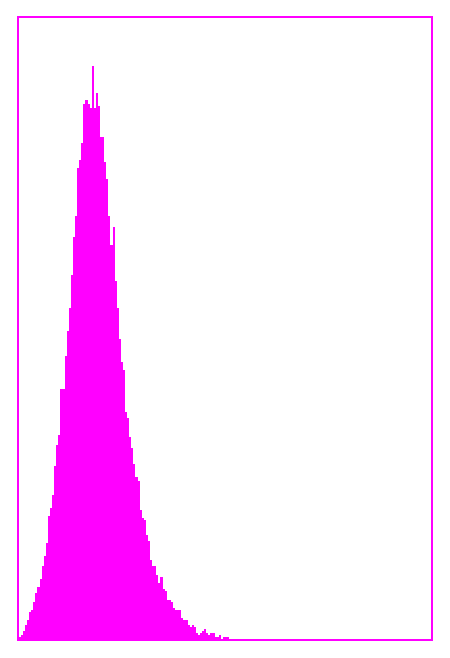
\includegraphics[width=1cm]{obrazky/dft_histogram}
            
\includegraphics[width=1cm]{obrazky/dct_histogram}
            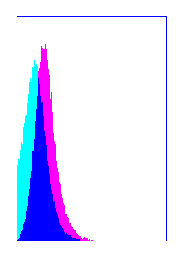
\includegraphics[width=1cm]{obrazky/combined_histogram}
        }
        \end{centering}
    \end{figure}
\end{frame}
%%% }}}

%%% {{{ Kompresia zvuku
\subsection{Kompresia zvuku}
\begin{frame}{Kompresia zvuku}
    \begin{itemize}
        \item Kompresia zvuku je náročnejšia ako obrazu
            \begin{itemize}
            \item problémy spracovania po úsekoch
            \item riešenie - windowing a modifikovaná transformácia
            \end{itemize}
    \end{itemize}
    \begin{figure}
        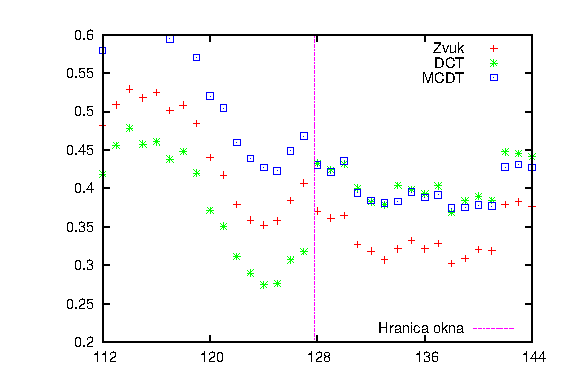
\includegraphics[width=5cm]{obrazky/dct_vs_mdct}
    \end{figure}
\end{frame}
%%% }}}

%%% {{{ Rychle nasobenie polynomov
%\subsection{Použitia v teoretickej informatike}
%\begin{frame}{Teoretická informatika}
%    \begin{itemize}
%        \item Odvodenie algoritmu na rýchle násobenie polynómov
%        \item Súvislosť násobenia polynómov s Fourierovou
%        transformáciou
%            \begin{itemize}
%                \item Všeobecná FT v poli resp. okruhu
%                \item Odvodený algoritmus - Radix2 FFT
%            \end{itemize}
%        \item hashovacie funkcie za pomoci FFT
%    \end{itemize}
%\end{frame}
%%% }}}


\section{Záver}
%%% {{{ Zhrnutie
\subsection{Zhrnutie}
\begin{frame}{Zhrnutie práce}
    \begin{itemize}
        \item Zjednotenie poznatkov o FT
            \begin{itemize}
                \item zosúladenie definícii
                \item zjednotenie dôkazov
            \end{itemize}
        \item Použitia FT v informatike
            \begin{itemize}
                \item rôzne použitia
                \item súvislosti medzi nimi
            \end{itemize}

    \end{itemize}
\end{frame}
%%% }}}

%%% {{{ Dalsia praca
\subsection{Ďalšia práca}
\begin{frame}{Ďalšia práca}
    \begin{itemize}
        \item Algoritmy na výpočet rýchlej Fourierovej transformácie
            \begin{itemize}
                \item Radix-2 rýchle algoritmy
                \item Cooley-Tukey pre zložené čísla
                \item Algoritmy pre prvočíselné dĺžky
            \end{itemize}
        \item Použitie v matematike
            \begin{itemize}
                \item Riešenie diferenciálnych rovníc
                \item Ortonormálne systémy
            \end{itemize}
        \item Použitie vo fyzike
            \begin{itemize}
                \item FTIR
                \item NMRI, CT
                \item Kvantová mechanika
            \end{itemize}
    \end{itemize}
\end{frame}
%%% }}}


%%% {{{ Koniec
\begin{frame}{Koniec}
    \begin{table}
    \begin{centering}
        \large Ďakujem za pozornosť.
    \end{centering}
    \end{table}
\end{frame}
%%% }}}

\end{document}
